\documentclass[11pt,a4paper]{article}

\usepackage[utf8x]{inputenc}
\usepackage[T1]{fontenc}

\usepackage{pdfpages}
\usepackage{palatino}
\usepackage{enumitem}
\usepackage{outlines} %support nested list
\usepackage{float}
\usepackage{framed}

\usepackage{desclist}

\usepackage{todonotes}
%Define the listing package
\usepackage{listings} %code highlighter
\usepackage{color} %use color
\definecolor{mygreen}{rgb}{0,0.6,0}
\definecolor{mygray}{rgb}{0.5,0.5,0.5}
\definecolor{mymauve}{rgb}{0.58,0,0.82}
 
%Customize a bit the look
\lstset{ %
 backgroundcolor=\color{white}, % choose the background color; you must add \usepackage{color} or \usepackage{xcolor}
 basicstyle=\footnotesize, % the size of the fonts that are used for the code
 breakatwhitespace=false, % sets if automatic breaks should only happen at whitespace
 breaklines=true, % sets automatic line breaking
 captionpos=b, % sets the caption-position to bottom
 commentstyle=\color{mygreen}, % comment style
 deletekeywords={...}, % if you want to delete keywords from the given language
 escapeinside={\%*}{*)}, % if you want to add LaTeX within your code
 extendedchars=true, % lets you use non-ASCII characters; for 8-bits encodings only, does not work with UTF-8
 frame=single, % adds a frame around the code
 keepspaces=true, % keeps spaces in text, useful for keeping indentation of code (possibly needs columns=flexible)
 keywordstyle=\color{blue}, % keyword style
% language=Octave, % the language of the code
 morekeywords={*,...}, % if you want to add more keywords to the set
 numbers=left, % where to put the line-numbers; possible values are (none, left, right)
 numbersep=5pt, % how far the line-numbers are from the code
 numberstyle=\tiny\color{mygray}, % the style that is used for the line-numbers
 rulecolor=\color{black}, % if not set, the frame-color may be changed on line-breaks within not-black text (e.g. comments (green here))
 showspaces=false, % show spaces everywhere adding particular underscores; it overrides 'showstringspaces'
 showstringspaces=false, % underline spaces within strings only
 showtabs=false, % show tabs within strings adding particular underscores
 stepnumber=1, % the step between two line-numbers. If it's 1, each line will be numbered
 stringstyle=\color{mymauve}, % string literal style
 tabsize=2, % sets default tabsize to 2 spaces
 title=\lstname % show the filename of files included with \lstinputlisting; also try caption instead of title
}
%END of listing package%

\setlist[itemize]{topsep=3pt,after=\vspace{.5\baselineskip}}
\usepackage[left=3cm,right=3cm,top=3cm,bottom=3cm]{geometry}
\setlength{\parskip}{2mm}


\def\blurb{\textsc{Université catholique de Louvain\\
  École polytechnique de Louvain\\
  Pôle d'ingénierie informatique}}
\def\clap#1{\hbox to 0pt{\hss #1\hss}}%
\def\ligne#1{%
  \hbox to \hsize{%
    \vbox{\centering #1}}}%
\def\haut#1#2#3{%
  \hbox to \hsize{%
    \rlap{\vtop{\raggedright #1}}%
    \hss
    \clap{\vbox{\vfill\centering #2\vfill}}%
    \hss
    \llap{\vtop{\raggedleft #3}}}}%
\begin{document}

\begin{titlepage}
\thispagestyle{empty}\vbox to 1\vsize{%
  \vss
  \vbox to 1\vsize{%
    \haut{\raisebox{-5mm}{
\includegraphics[width=2.5cm]{img/logo_ucl.pdf}}}{\blurb}{\raisebox{-5mm}{
\includegraphics[scale=0.20]{img/ingi_logo.png}}}
    \vfill
    \ligne{\Huge \textbf{\textsc{LINGI2251}}}
     \vspace{5mm}
    \ligne{\huge \textbf{\textsc{Software Engineering: Development Methods}}}
     \vspace{15mm}
    \ligne{\Large \textbf{\textsc{Assignment 2}}}
    \vspace{5mm}
    \ligne{\large{\textsc{12 april 2016}}}
    \vfill
    \vspace{5mm}
    \ligne{%
         \textsc{Alexandre Hauet\\Tanguy Vaessen} 
      }
      \vspace{5mm}
    }%
  \vss
  }
\end{titlepage}

%\tableofcontents

\section{Architectural Design}
\subsection{Hierarchical decomposition}

\begin{figure}[H]
 \centering
 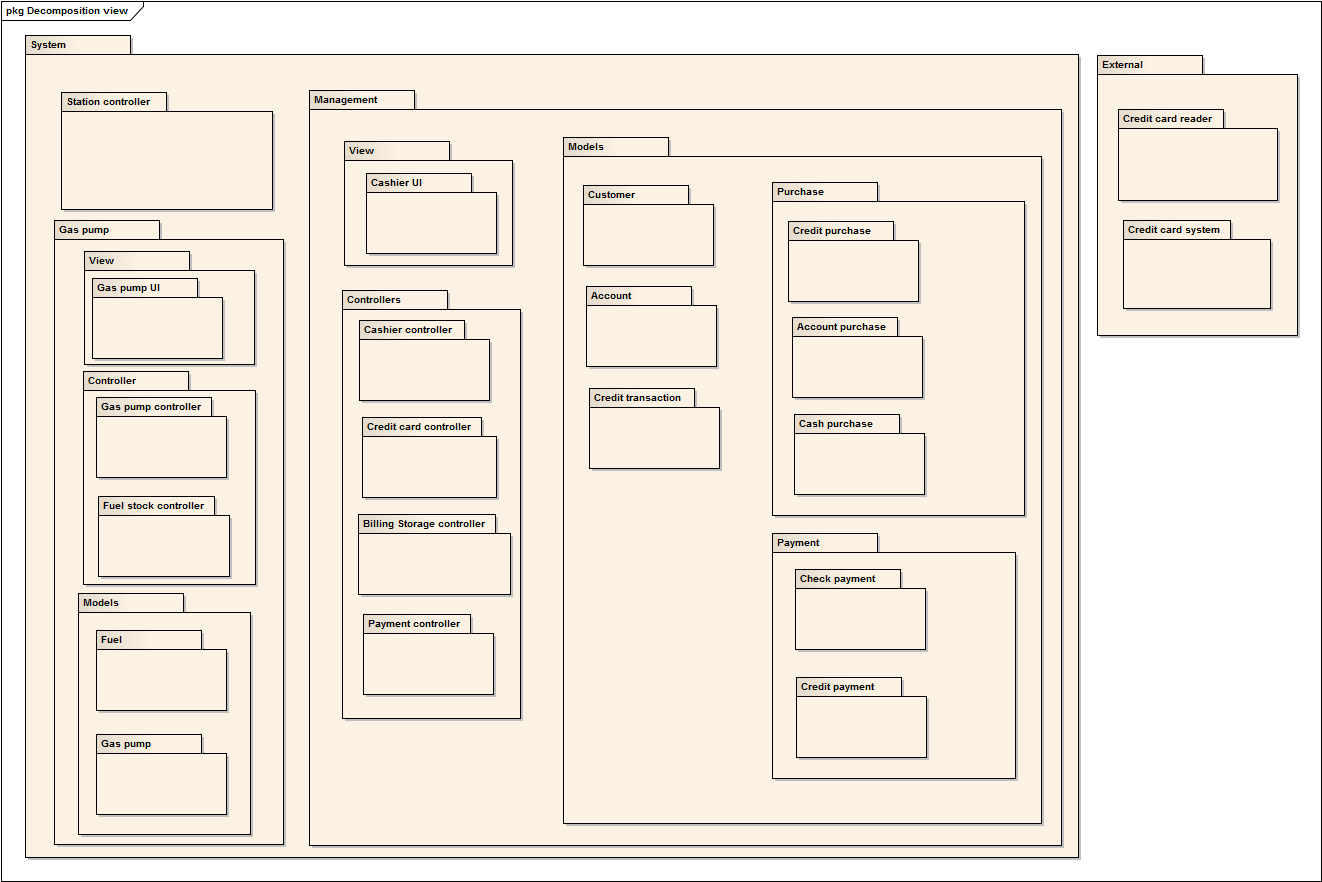
\includegraphics[width=\textwidth]{../DecompositionView.png} 
 \caption{Hierarchical decomposition}
 \label{fig:dep}
\end{figure}

\subsection{Roles and interactions of all components}

Our system is composed of three parts. The first is the station controller which control all the station. The second is the Gas Pump which is about the logistic of the pump. And finally, the Management part which allow to customers to pay or to manage the billing.

\subsubsection*{Station controller}

\subsubsection*{Gas Pump}
\begin{itemize}
\item{Gaz pump UI :} Interface with which the user interacts.
\item{Gaz pump controller :} Control the different interaction between the system (Station controller) and the different elements of the Gas pumps.
\item{Fuel stock controller :} Manage the stock of fuel of the station.
\item{Fuel :} Represent a specific type of fuel.
\item{Gaz pump :} Deliver the gaz to the costumers and compute the accounting. 
\end{itemize}
\subsubsection*{Management}
\begin{itemize}
\item{Cashier UI :} Interface with which the user interacts.
\item{Cashier controller :} Allow the interaction between the cashier system and the global system (Station controller).
\item{Credit card controller :} Manage the interaction between the external credit card system and our system.
\item{Billing storage controller :} Manage the billing accounts.
\item{Payment controller :} Handle the customer to pay.
\item{Customer :} Represent a customer with the different fields needed
\item{Account :} Compute the account of a purchase
\item{Credit transaction :}
\item{Credit payment :}
\item{Credit purchase :}
\item{Account purchase :}
\item{Cash purchase :}
\end{itemize}

\section{Detailed Design}
\subsection{Class diagram}

\begin{figure}[H]
 \centering
 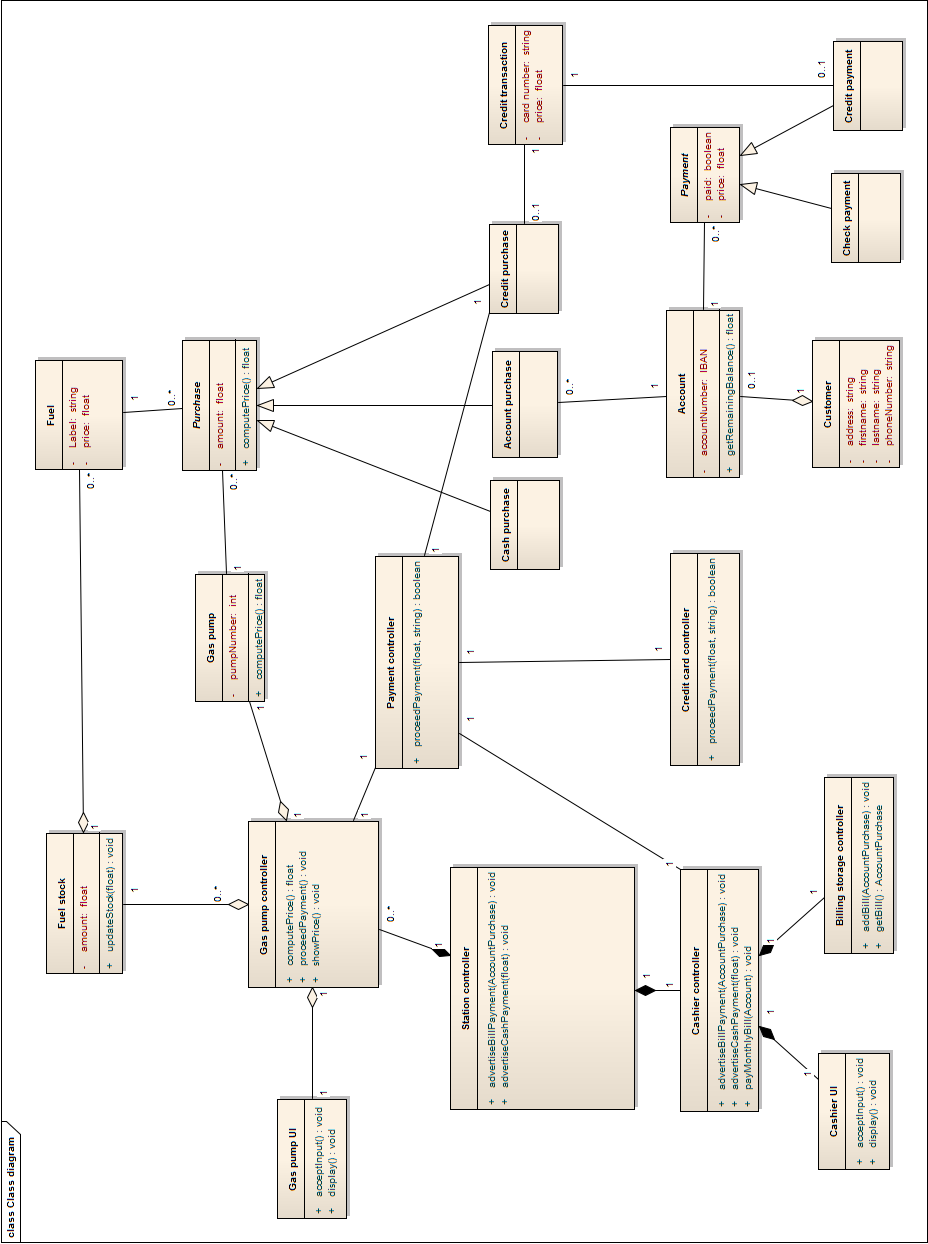
\includegraphics[width=\textwidth]{../ClassDiagram.png} 
 \caption{Class diagram}
 \label{fig:dep}
\end{figure}

\end{document}
